% ==============================================================================
% PAGE 29: 11) SOLAR PANEL UNIT (Numbered Page 21)
% ==============================================================================
\subsubsection*{11) SOLAR PANEL UNIT}

\begin{center}
  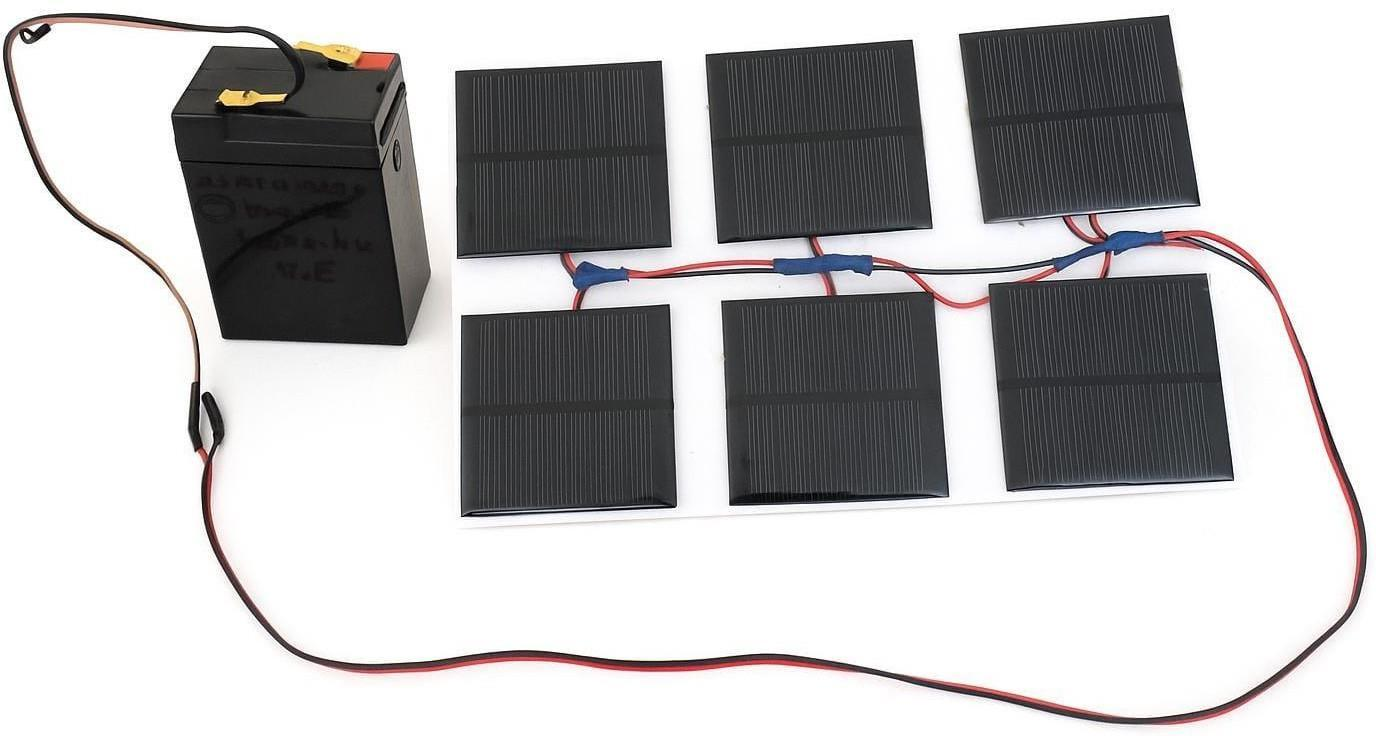
\includegraphics[width=90mm]{figures/fig13_solar_panel_unit.jpg}
\end{center}

\noindent
\begin{spacing}{1.2}
{\fontsize{10.2}{14.5}\selectfont
A solar panel unit is used as the main source of electrical power generation. Each solar panel is capable of producing around 6 amperes of current, and when connected together in a suitable configuration, the entire system generates a total output voltage of about 10 to 12 volts. This generated DC power is used for charging the battery, which later supplies energy to the control and motor units of the system. Solar energy is a renewable and eco-friendly source, making the setup efficient and sustainable for long-term operation.\\[3mm]
To ensure safe operation, a diode is connected in the circuit to allow one-way power flow from the solar panels to the battery. This prevents the reverse flow of current, protecting the solar panels from short-circuiting or back current during low or no sunlight conditions. This arrangement helps maintain the reliability and safety of the charging system.
}
\end{spacing}
\clearpage
